 \documentclass{article}
 \usepackage[T1]{fontenc}
 \usepackage{graphicx}
 \usepackage{lipsum} % produce dummy text as filler
 \usepackage{float}
 \usepackage{trivfloat}
 \trivfloat{image}
 \graphicspath{{figs/}}



 \begin{document}

\section{Including Graphics}
 \subsection{Altering graphic appearance}
 This picture
 \begin{center}
 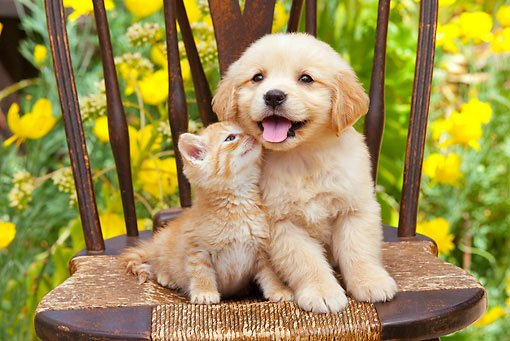
\includegraphics[height=2cm]{pic}
 \end{center}
Size


 \begin{center}
 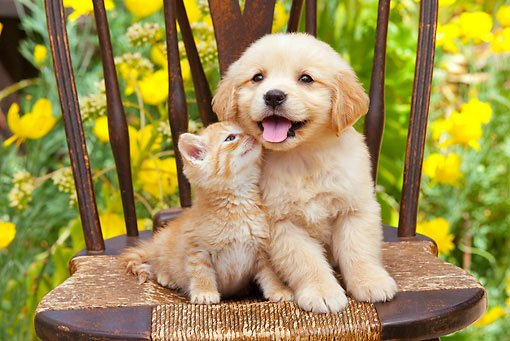
\includegraphics[height = 0.3\textheight]{pic}
 \end{center}
 Some text
 \begin{center}
 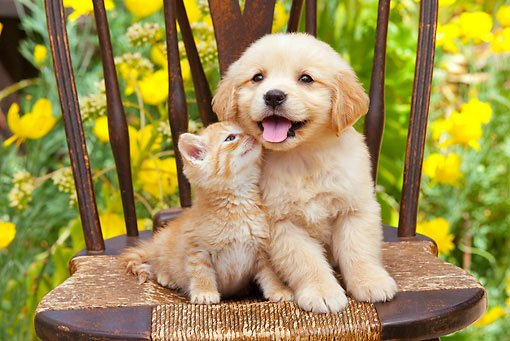
\includegraphics[width = 0.9\textwidth]{pic}
 \end{center}

\begin{center}
 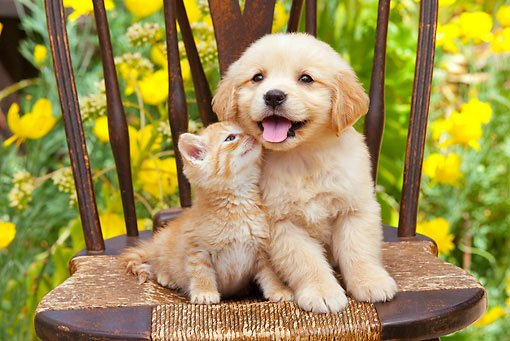
\includegraphics[scale=0.6,angle=20]{pic}
 \end{center}


\begin{center}
 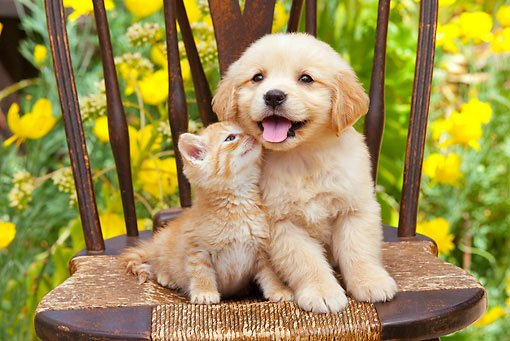
\includegraphics[clip, trim = 50 25 50 30]{pic}
 \end{center}

 \subsection{ Making images float}

\lipsum[1-4] % Just a few filler paragraphs
 Test location.
 \begin{figure}[ht]
 \centering
 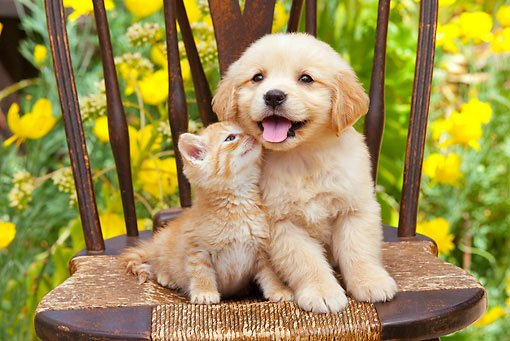
\includegraphics[width=0.7\textwidth]{pic.jpg}
 \caption{An example image}

 \end{figure}
 \lipsum[6-10] % Just a few filler paragraphs

 \subsection{  Placing floats}

 \lipsum[1-7]
 \begin{figure}[H]
 \centering
 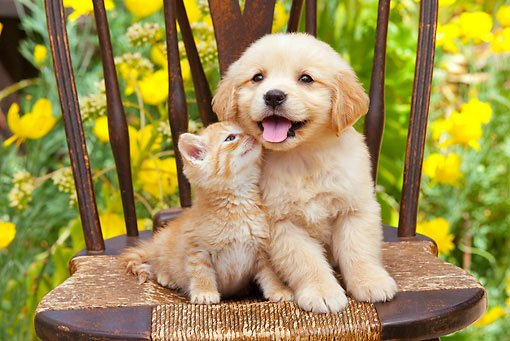
\includegraphics[width=0.7\linewidth]{pic}
 \caption{An example image}
 \end{figure}
 \lipsum[8-15]

 \subsection{Other types of float}

 \begin{image}
 \centering
 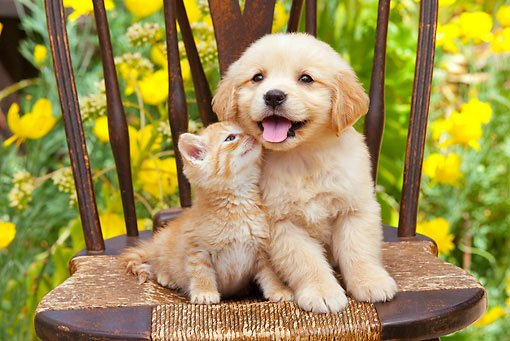
\includegraphics[width=0.5\textwidth]{pic}
 \caption{An example image}
 \end{image}

 \subsection{Cross-referencing}

 Hey world!
 This is a first document.
 \section{Title of the second section}
 Text of material for the first section.
 \subsection{Subsection of the second section}
 \label{subsec:labelone}
 Text of material for the first subsection.
 \begin{equation}
 e^{i\pi}+1 = 0
 \label{eq:labeltwo}
 \end{equation}
 In subsection~\ref{subsec:labelone} is
 equation~\ref{eq:labeltwo}.

 \section{Introduction}
 Some exciting text with a reference~\ref{sec:next}.
 \section{Next thing}
 \label{sec:next}
 More text here.



\lipsum[1-4] % Just a few filler paragraphs
 Test location.
 \begin{figure}[b]
 \centering
 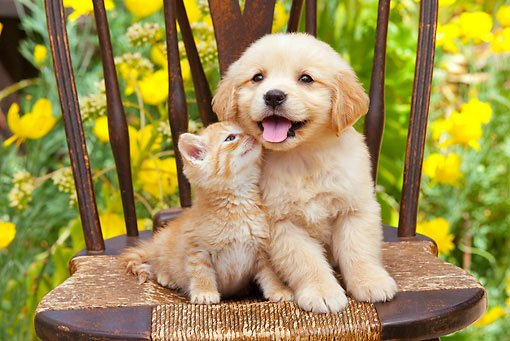
\includegraphics[width=0.5\textwidth]{pic.jpg}
 \caption{An example image}
 \end{figure}
 \lipsum[6-10] % Just a few filler paragraphs
 \end{document}